\documentclass[11pt]{article}

\usepackage[margin=1in]{geometry}
\usepackage[T1]{fontenc}
\usepackage[utf8]{inputenc}
\usepackage{newtxtext,newtxmath}
\usepackage{hyperref}
\usepackage{graphicx}
\usepackage{booktabs}
\usepackage{longtable}
\usepackage[backend=biber,style=numeric,sorting=none]{biblatex}

\addbibresource{references.bib}

\hypersetup{
    colorlinks=true,
    linkcolor=black,
    urlcolor=blue
}

\begin{document}


\begin{center}
    {\LARGE\bfseries Replicating a Spherical Fuzzy SWARA--EDAS Framework for Pedestrian Safety in Bus Rapid Transit Systems}

    \vspace{0.5em}

    {\large A From-Scratch Reproduction of Ayyildiz et al. (2026)}

    \vspace{1em}

    Augustine Stevis Agoha -- 22425046\\
    Marvin Kabutey -- 22425067\\
    Theophilus Caesar -- 22424543
\end{center}

\vspace{1em}
% -------------------------------------------------------
\section*{Abstract}
% -------------------------------------------------------
This report documents the implementation and reproduction of the decision-making framework proposed by Ayyildiz et al. (2026) in \emph{Decision-Making Framework for Pedestrian Safety Optimisation in Bus Rapid Transit Systems} from scratch. The study integrates Spherical Fuzzy Stepwise Weight Assessment Ratio Analysis (SF-SWARA) and Spherical Fuzzy Evaluation based on Distance from Average Solution (SF-EDAS) to prioritise pedestrian safety interventions for Bus Rapid Transit (BRT) systems. With no referenced implementation provided, the complete framework---including spherical fuzzy number operations, the Spherical Weighted Arithmetic Mean (SWAM) aggregation operator, SF-SWARA criterion weighting, SF-EDAS strategy evaluation, and validation procedures---was implemented directly from the mathematical formulations presented in the paper.

Validation was carried out against the published intermediate and final results wherever possible. The implementation, to a notable degree, successfully reproduced the published SF-SWARA score values, criterion ranking, and the final ranking of candidate strategies, identifying awareness campaigns and pedestrian traffic enforcement as the highest-priority intervention. Numerical differences were observed in several intermediate computations, including criterion weights, aggregated decision matrix values, positive and negative distance matrices and final appraisal scores. These differences did not alter the overall prioritisation of strategies and are discussed as potential consequences of implementation ambiguities, undocumented assumptions, or numerical conventions that could not be fully inferred from the published methodology.

The project demonstrates that the proposed SF-SWARA--SF-EDAS framework can be implemented independently and used to reproduce the study's principal decision-making outcomes while highlighting the importance of transparent reporting and comprehensive validation in computational research.

% -------------------------------------------------------
\section{Introduction}
% -------------------------------------------------------
Bus Rapid Transit (BRT) systems have become an increasingly popular solution for improving urban mobility by providing high-capacity public transport at a lower cost than conventional rail systems. Despite delivering notable operational efficiencies, BRT corridors present considerable pedestrian safety concerns. The presence of exclusive bus lanes, complex pedestrian crossing facilities, high vehicular traffic volumes, and frequent pedestrian--vehicle interactions collectively increase exposure to conflict points, thereby elevating the risk of pedestrian crashes.

Identifying the most appropriate pedestrian safety intervention represents a complex multi-criteria decision-making (MCDM) problem involving the assessment of multiple safety criteria simultaneously. Candidate interventions must be evaluated against these criteria without discarding uncertainty in expert judgements. Conventional MCDM techniques typically employ precise numerical values, which may not adequately capture the ambiguity inherent in human evaluations. Spherical Fuzzy Sets offer a more adaptable approach by representing each assessment through independent degrees of membership, non-membership, and hesitancy, thereby incorporating uncertainty directly into the decision-making process.

The work reproduced in this project is based on the framework proposed by Ayyildiz et al. (2026) \cite{ayyildiz2026}, which combines Spherical Fuzzy Stepwise Weight Assessment Ratio Analysis (SF-SWARA) and Spherical Fuzzy Evaluation based on Distance from Average Solution (SF-EDAS) to prioritise pedestrian safety interventions along the Dar es Salaam Bus Rapid Transit corridor. Within the framework, SF-SWARA is used to determine the relative importance of pedestrian safety criteria, while SF-EDAS evaluates competing intervention strategies using the previously derived criterion weights.

The primary objective of this project was not to improve or modify the proposed methodology but to reproduce it as faithfully as possible using an independent implementation developed entirely from the published mathematical formulations. Since no official source code or reference implementation accompanies the paper, every component of the framework---including spherical fuzzy number operations, aggregation operators, criterion weighting, strategy evaluation, validation routines, and sensitivity analysis---has been implemented from scratch. The implementation was then validated against the intermediate values and final results reported in the paper to assess the extent to which the published methodology could be reproduced.

Beyond replicating the principal findings of the original study, this project undertakes a broader assessment of the reproducibility of complex fuzzy multi-criteria decision-making (MCDM) research. A systematic comparison between independently generated results and the published values is conducted to determine the extent to which the proposed framework can be reproduced in an independent implementation. This analysis not only confirms the strengths and reliability of the methodological framework but also exposes the practical difficulties encountered when computational research lacks sufficient methodological transparency and detailed implementation specifications. The findings underscore the importance of comprehensive documentation for ensuring reproducibility and facilitating future research.

% -------------------------------------------------------
\section{Methodology Overview}
% -------------------------------------------------------
The implemented framework follows the two-stage decision-making process proposed by Ayyildiz et al. (2026). The first stage determines the relative importance of the evaluation criteria using Spherical Fuzzy Stepwise Weight Assessment Ratio Analysis (SF-SWARA), while the second stage ranks the candidate pedestrian safety strategies using Spherical Fuzzy Evaluation based on Distance from Average Solution (SF-EDAS). Both stages operate entirely within the spherical fuzzy environment and utilise the Spherical Weighted Arithmetic Mean (SWAM) operator to aggregate the opinions of multiple experts.

Figure~\ref{fig:workflow} illustrates the overall workflow implemented in this project.

\begin{figure}[h]
    \centering
    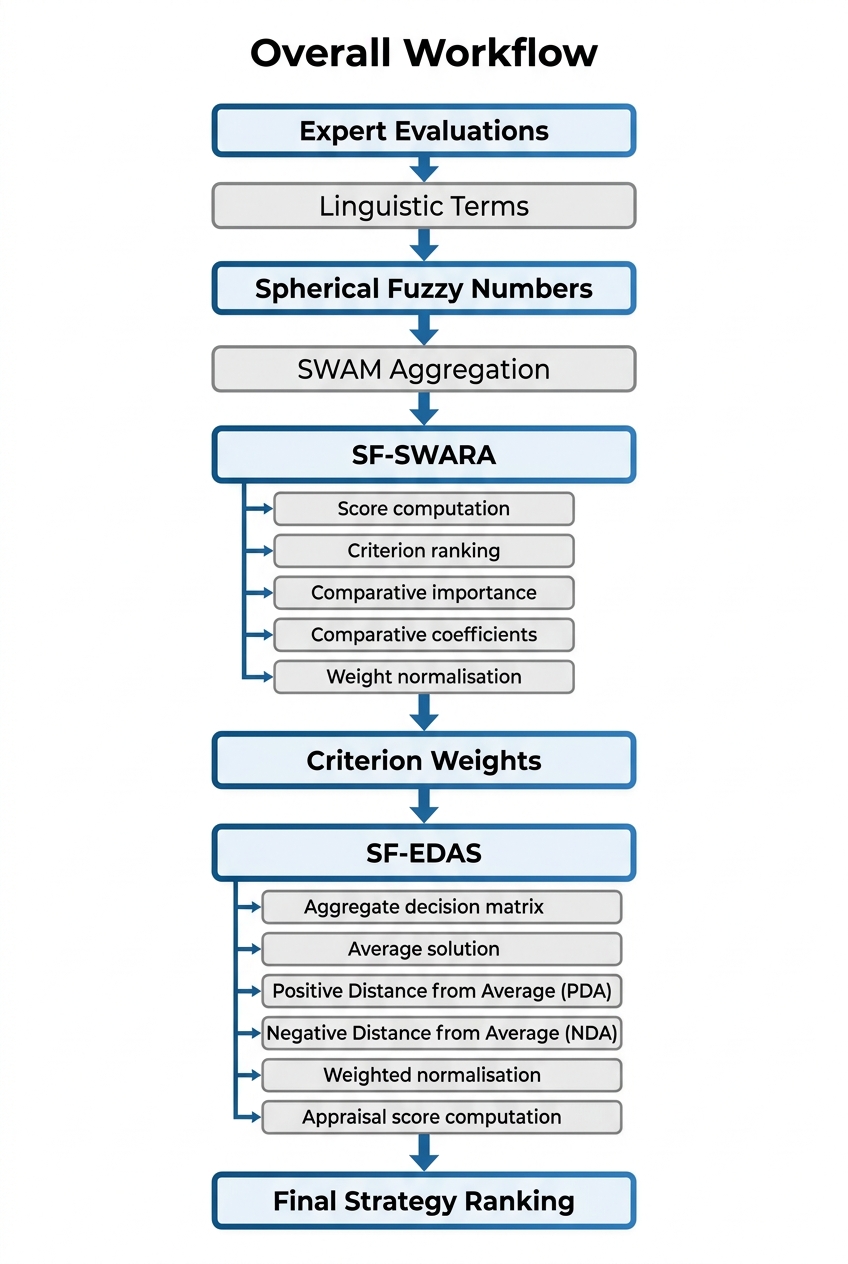
\includegraphics[width=0.4\textwidth]{technical_flowchart_diagram.png}
    \caption{Overall workflow implemented in this project.}
    \label{fig:workflow}
\end{figure}

\subsection{Stage 1 --- SF-SWARA}
The primary objective of the first stage is to determine the relative importance of each pedestrian safety criterion. Expert assessments are first expressed using predefined linguistic terms (nine terms, from ``Extremely Low'' to ``Extremely High''), which are mapped to spherical fuzzy numbers consisting of membership, non-membership, and hesitancy values.

The individual expert evaluations are then combined using the Spherical Weighted Arithmetic Mean (SWAM) operator to produce a single aggregated spherical fuzzy evaluation for each criterion. These aggregated values are converted into precise scores using the score function defined in the paper. The criteria are subsequently ranked according to these scores, after which the SF-SWARA procedure computes comparative importance values, comparative coefficients, recalculated weights and finally, normalised criterion weights whose sum equals one.

The resulting criterion weights quantify the relative influence of each safety challenge and are subsequently used during strategy evaluation.

\subsection{Stage 2 --- SF-EDAS}
The second stage evaluates the alternative pedestrian safety strategies using the criterion weights obtained from SF-SWARA.

Each strategy is assessed against every criterion by multiple experts using the same linguistic scale. These evaluations are aggregated using the SWAM operator to form a collective spherical fuzzy decision matrix. An average solution is then computed for each criterion, representing the overall reference point against which all strategies are compared.

For every strategy, Positive Distance from Average (PDA) and Negative Distance from Average (NDA) values are calculated according to the mathematical definitions provided in the original framework. These distance measures are weighted using the criterion weights from Stage 1, normalised across all alternatives, and combined to produce a final appraisal score for each strategy.

These appraisal scores determine the final ranking of the candidate pedestrian safety interventions.

\subsection{Case Study Data}
The implementation uses the case study presented in the original paper, which considers five pedestrian safety criteria, three candidate intervention strategies, and four domain experts. All expert assessments and linguistic evaluations were transcribed directly from the supplementary material accompanying the publication and stored in structured CSV files for reproducibility. These datasets serve as the sole inputs to the implementation and allow direct comparison between the computed results and the published values reported by the authors.

% -------------------------------------------------------
\section{Implementation Approach}
% -------------------------------------------------------
The objective of this project was to develop an independent implementation of the SF-SWARA--SF-EDAS decision-making framework directly from the mathematical formulations presented by Ayyildiz et al. (2026). As no reference implementation or source code accompanied the publication, every component of the framework was implemented using Python.

Development followed a structured, incremental approach. Before implementation began, the paper and its supplementary material were studied in detail, all mathematical equations were documented, and the required datasets were extracted into structured CSV files. Each equation was then implemented individually and validated before progressing to the next stage of the framework. This iterative workflow reduced the likelihood of propagating errors through subsequent computations and simplified debugging.

To improve maintainability and traceability, the implementation was organised into independent modules, each responsible for a specific stage of the computational pipeline.

\begin{longtable}{p{0.22\textwidth}p{0.68\textwidth}}
\toprule
\textbf{Module} & \textbf{Responsibility} \\
\midrule
\endhead
\texttt{models.py} & Defines the \texttt{SphericalFuzzyNumber} data model and core data structures used throughout the implementation. \\
\texttt{loader.py} & Loads and parses the case-study datasets and linguistic evaluation tables from CSV files. \\
\texttt{spherical\_fuzzy.py} & Implements spherical fuzzy number operations, score calculations, and supporting mathematical utilities. \\
\texttt{swam.py} & Implements the Spherical Weighted Arithmetic Mean (SWAM) operator used to aggregate expert evaluations. \\
\texttt{sf\_swara.py} & Implements the complete SF-SWARA criterion-weighting procedure, including score computation, criterion ranking, comparative importance, coefficient calculation, recursive weight computation, and weight normalisation. \\
\texttt{sf\_edas.py} & Implements the SF-EDAS strategy evaluation procedure, including decision matrix aggregation, average solution computation, PDA/NDA calculation, weighted normalisation, appraisal score computation, and strategy ranking. \\
\texttt{validation.py} & Compares computed intermediate and final results against the published values reported in the paper to assess implementation accuracy. \\
\texttt{main.py} & Coordinates the execution of the complete pipeline and produces the final outputs. \\
\bottomrule
\caption{Python scripts and brief description.}
\label{tab:modules}
\end{longtable}

The modular architecture ensured that each stage of the framework could be implemented, tested, and validated independently while maintaining clear separation of responsibilities. This also simplified debugging by allowing intermediate outputs to be inspected before they were used as inputs to subsequent stages.

Implementation was guided directly by the published equations rather than attempting to reproduce the reported numerical results through empirical adjustment. Each computational stage was verified against the corresponding values presented in the paper wherever possible, allowing discrepancies to be identified and investigated systematically.

The completed implementation reproduces the full computational workflow described in the original study, from the conversion of linguistic evaluations into spherical fuzzy numbers through to the generation of final strategy rankings. The modular design also allows individual components, such as the SWAM aggregation operator, SF-SWARA weighting procedure, and SF-EDAS evaluation procedure, to be reused independently in future multi-criteria decision-making applications.

% -------------------------------------------------------
\section{Validation Process}
% -------------------------------------------------------
Validation was performed throughout the implementation rather than only after the complete framework had been developed. Each major computational stage was verified independently against the corresponding intermediate or final results reported in the original paper. This incremental validation strategy helped isolate discrepancies, confirm the correctness of individual algorithms, and reduce the propagation of implementation errors through later stages of the decision-making pipeline.

The validation process focused on both intermediate computations and final outputs. The following components were evaluated:

\begin{itemize}
    \item SF-SWARA score values.
    \item Criterion ranking.
    \item Normalised criterion weights.
    \item Aggregated spherical fuzzy decision matrix.
    \item Positive Distance from Average (PDA) values.
    \item Negative Distance from Average (NDA) values.
    \item Final appraisal scores.
    \item Final strategy ranking.
\end{itemize}

Where published intermediate values were available, the implementation outputs were compared directly against the corresponding tables presented in the paper. Numerical comparisons were performed using appropriate tolerances to account for the rounding precision used in the published results. Table~\ref{tab:validation} summarises the validation outcomes.

\begin{table}[h]
    \centering
    \begin{tabular}{ll}
        \toprule
        \textbf{Component} & \textbf{Validation Outcome} \\
        \midrule
        SF-SWARA score values & Reproduced successfully. \\
        Criterion ranking & Reproduced successfully. \\
        Normalised criterion weights & Numerical differences observed. \\
        Aggregated decision matrix & Minor numerical differences observed in some values. \\
        PDA matrix & Numerical differences observed. \\
        NDA matrix & Numerical differences observed. \\
        Final appraisal scores & Numerical differences observed. \\
        Final strategy ranking & Reproduced successfully (S2 > S1 > S3). \\
        \bottomrule
    \end{tabular}
    \caption{Component and validation outcome.}
    \label{tab:validation}
\end{table}

The validation results indicate that the implementation successfully reproduces the principal decision-making behaviour of the published framework. In particular, the criterion ordering obtained from the SF-SWARA procedure matches the published ranking exactly, and the final SF-EDAS evaluation identifies the same highest-ranked pedestrian safety strategy as reported in the original study.

Although numerical differences were observed in several intermediate computations, these differences did not alter the final prioritisation of strategies. The discrepancies are therefore reported and discussed rather than concealed, since they may arise from implementation ambiguities, undocumented numerical conventions, rounding behaviour, or assumptions that are not explicitly described in the published methodology. Without access to the authors' original implementation, the precise source of these differences cannot be determined conclusively.

Overall, the validation demonstrates that the developed implementation faithfully reproduces the methodology and principal findings of the original study while providing a transparent account of the intermediate computations that differed from the published values.

% -------------------------------------------------------
\section{Results}
% -------------------------------------------------------
The developed implementation successfully executed the complete SF-SWARA--SF-EDAS framework using the case study and expert evaluation data provided in the original publication. Results were generated for every stage of the computational pipeline, including criterion weighting, strategy evaluation, and final ranking.

\subsection{Criterion Evaluation}
The application of the SF-SWARA procedure produced the same ordering of pedestrian safety criteria reported in the original study. The criterion relating to the absence of special consideration for children crossing the road received the highest importance ranking, followed by the remaining criteria in the same order, matching the paper's finding and its discussion of comparable results from Lagos and Johannesburg BRT corridors.

The score values computed during the SF-SWARA stage were successfully reproduced, confirming the correctness of the spherical fuzzy score function and the implementation of the early stages of the weighting procedure. Although the final normalised criterion weights differed numerically from those reported in the paper, the relative ordering of criterion importance remained unchanged.

\subsection{Strategy Evaluation}
The SF-EDAS procedure was subsequently applied using the criterion weights obtained from the first stage. Aggregated decision matrices, average solutions, positive and negative distance measures, weighted distances, and appraisal scores were computed for each candidate intervention strategy.

Minor numerical differences were observed in several intermediate calculations when compared with the published values. Despite these differences, the implementation consistently identified the same highest-ranked strategy reported in the original study.

The computed strategy ranking was:

\begin{table}[h]
    \centering
    \begin{tabular}{cl}
        \toprule
        \textbf{Rank} & \textbf{Strategy} \\
        \midrule
        \textbf{1} & Awareness campaigns and fines for pedestrians who violate traffic rules (S2) \\
        \textbf{2} & Relocating Bus Rapid Transit lanes off the roadway (S1) \\
        \textbf{3} & Special design and operational considerations for vulnerable road users (S3) \\
        \bottomrule
    \end{tabular}
    \caption{Component and validation outcome.}
    \label{tab:ranking}
\end{table}

This ranking matches the ordering reported in the original paper.

\subsection{Overall Reproduction}
The implementation successfully reproduced the principal decision-making outcomes of the published framework. In particular:

\begin{itemize}
    \item The SF-SWARA score values were reproduced successfully.
    \item The criterion ranking matched the published results exactly.
    \item The final strategy ranking matched the published results exactly.
    \item The highest-priority pedestrian safety intervention remained awareness campaigns combined with enforcement measures.
\end{itemize}

Numerical differences were observed in several intermediate stages of the computation, including criterion weights, portions of the aggregated decision matrix, PDA and NDA values, and final appraisal scores. However, these differences did not affect the overall prioritisation of the alternative strategies.

These results demonstrate that the independently developed implementation captures the behaviour of the published decision-making framework and reproduces its principal conclusions while highlighting areas where intermediate numerical values differ from those presented in the paper.

% -------------------------------------------------------
\section{Discussion}
% -------------------------------------------------------
The objective of this project was to reproduce the published SF-SWARA--SF-EDAS framework as faithfully as possible rather than to modify or improve the methodology. Validation therefore focused not only on reproducing the final decision but also on comparing intermediate computational results with those reported in the original study.

The implementation successfully reproduced several key components of the published framework, including the SF-SWARA score values, the ranking of pedestrian safety criteria, and the final ranking of the candidate intervention strategies. These outcomes demonstrate that the overall computational workflow and decision-making behaviour of the framework were successfully replicated.

Despite reproducing the principal findings, numerical differences were observed in several intermediate stages of the computation. These differences included the normalised criterion weights, portions of the aggregated spherical fuzzy decision matrix, the Positive Distance from Average (PDA) and Negative Distance from Average (NDA) matrices, and the final appraisal scores. Although these numerical deviations propagated through later stages of the framework, they did not alter the final ordering of the alternative strategies.

Several factors may contribute to these differences. The published paper provides the mathematical formulation of the framework but omits certain implementation details that can influence numerical results. Examples include floating-point precision, rounding conventions, intermediate calculation precision, implementation-specific interpretations of recursive computations, and assumptions that are not explicitly documented in the methodology. Small differences introduced during early stages of the computation may accumulate as later calculations build upon previous results.

Since no official implementation or reference source code accompanies the publication, it is not possible to determine conclusively whether the observed differences originate from implementation choices, undocumented computational conventions, or aspects of the methodology that are not fully described in the paper. Consequently, this study does not claim that the published results are incorrect. Instead, it documents the observed differences transparently while demonstrating that the principal decision-making outcomes remain unchanged.

From a reproducibility perspective, these findings reinforce the importance of comprehensive reporting in computational research. Publishing source code, implementation details, and complete computational workflows alongside mathematical formulations would greatly improve the reproducibility of complex multi-criteria decision-making methods and enable more precise validation by independent researchers.

Overall, the implementation demonstrates that the SF-SWARA--SF-EDAS framework can be reproduced successfully using only the published methodology while also highlighting the practical challenges that arise when reproducing research in the absence of reference implementations.

% -------------------------------------------------------
\section{Challenges Encountered}
% -------------------------------------------------------
Several practical and technical challenges were encountered during the implementation of the SF-SWARA--SF-EDAS framework. Addressing these challenges was an important part of the replication process and contributed to a deeper understanding of both the methodology and its implementation.

\subsection{Development Environment}
The implementation was carried out using Python within a Windows Subsystem for Linux (WSL) environment. As the development environment was initially unconfigured, the required Python ecosystem and project dependencies had to be established before implementation could begin. Once configured, the environment provided a stable and reproducible platform for development and testing.

\subsection{Translating Mathematical Formulations into Code}
One of the primary challenges was translating the mathematical notation presented in the paper into reliable and maintainable software. Although the published equations describe the overall methodology, converting them into executable code required careful interpretation of recursive computations, aggregation operators, and spherical fuzzy number operations. To minimise implementation errors, each equation was implemented and validated individually before being integrated into the complete computational pipeline.

\subsection{Limited Implementation Detail}
The original publication provides the mathematical framework but does not include reference source code or detailed implementation guidelines. Consequently, several implementation decisions---such as data representation, numerical precision, and software architecture---had to be made independently while remaining faithful to the published methodology. Validation against the reported intermediate results was used to assess the reasonableness of these decisions throughout development.

\subsection{Validation of Intermediate Results}
A further challenge involved validating intermediate computational stages rather than relying solely on the final strategy ranking. The implementation produced numerical differences in some intermediate values despite reproducing the published criterion ordering and final strategy ranking. Investigating these differences required repeated verification of the input data, mathematical formulations, and software implementation to ensure that the observed discrepancies were documented accurately and were not the result of programming errors.

% -------------------------------------------------------
\section{Limitations}
% -------------------------------------------------------
While the implementation successfully reproduces the principal decision-making outcomes of the published SF-SWARA--SF-EDAS framework, several limitations should be acknowledged.

First, this study is based exclusively on the case study and expert evaluation data provided by Ayyildiz et al. (2026). The implementation was validated using the published datasets and was not evaluated on additional pedestrian safety case studies or alternative multi-criteria decision-making problems. Consequently, the generalisability of the implementation beyond the reported case study was not investigated within the scope of this project.

Second, the implementation relies solely on the methodological descriptions and mathematical formulations presented in the original publication. As no official source code or reference implementation was available, certain implementation decisions were made based on reasonable interpretations of the published methodology. Although these decisions were validated against the reported results wherever possible, they may differ from those adopted by the original authors.

Furthermore, several intermediate numerical results differed from those reported in the paper. While these differences did not affect the reproduced criterion ordering or final strategy ranking, the absence of a reference implementation makes it impossible to determine the precise source of these discrepancies. As a result, the study reports the observed differences without attributing them to either the implementation or the published work.

Finally, this project focuses exclusively on reproducing the SF-SWARA and SF-EDAS framework described in the paper. Other spherical fuzzy multi-criteria decision-making techniques, such as SF-TOPSIS and SF-VIKOR, were not implemented or compared, as they fall outside the objectives of this replication study.

Future work could evaluate the implementation using additional datasets, compare its performance with alternative spherical fuzzy MCDM methods, and investigate the computational performance of the framework on larger decision-making problems involving more criteria, alternatives, and experts.

% -------------------------------------------------------
\section{Conclusion}
% -------------------------------------------------------
This project presented a from-scratch implementation and reproduction of the SF-SWARA--SF-EDAS decision-making framework proposed by Ayyildiz et al. (2026) for prioritising pedestrian safety interventions in Bus Rapid Transit systems. Using only the published methodology and supplementary data, the complete computational framework was implemented in Python, including spherical fuzzy number operations, SWAM aggregation, SF-SWARA criterion weighting, SF-EDAS strategy evaluation, validation procedures, and supporting software modules.

Validation demonstrated that the implementation successfully reproduced the published SF-SWARA score values, the ranking of the evaluation criteria, and the final ranking of the alternative pedestrian safety strategies. Although numerical differences were observed in several intermediate computations, including criterion weights, aggregated decision matrix values, PDA/NDA matrices, and appraisal scores, these differences did not alter the principal decision-making outcomes reported in the original study.

Beyond reproducing the published methodology, the project demonstrates the feasibility of independently implementing complex spherical fuzzy multi-criteria decision-making frameworks in the absence of reference source code. The modular software architecture and systematic validation process also provide a reusable foundation for future applications of spherical fuzzy MCDM techniques in transportation and other decision-support domains.

Overall, the project achieved its primary objective of reproducing the published decision-making framework while providing a transparent evaluation of its implementation. The work highlights the importance of reproducibility, comprehensive validation, and clear methodological reporting in computational research, and provides a practical reference for future studies involving spherical fuzzy decision-making methods.

% -------------------------------------------------------
\section{References}
% -------------------------------------------------------

\printbibliography[heading=none]

\end{document}
